	\chapter{Web testing}
	\label{ch:Webtesting}

		There are several approaches for Web testing, the choice among them depends on
		different factors such as lifecycle of the project, technologies used, the
		budget, the professional level of developers. Two main ideas are Capture and
		Replay tests (C\&R) and programmable tests.
		
		\section{Capture and Replay}
		\label{sec:captureReplay}
			C\&R Web testing is based on capture/replay automated
			tools. \cite{CaptureReplay7} The software tester works with the Web
			application modeling user behaviour, the capture/replay tool records the
			whole session and generates the script, which can be executed later,
			repeating same actions without humans participation. Script editing might
			 be useful to adjust failed scripts accordingly
			to the changes of the Web page. Thought if the Web page was changed
			significantly, editing test script might be more expensive than recording the
			test from scratch. 
			
			We must admit that C\&R approach is very popular, there are plenty of
			frameworks both for desktop and Web applications such as TPTP GUI Recorder, SWTBot, QF-Test,
			Selenium IDE.
			The main advantage of this method of testing, is that the tester does not
			require to have experience in coding and building test cases with such tools is a simple task. 
			
			On the contrary, maintaining tests is harder and more expensive.
			The main problem is that editing generated scripts is harder than editing
			scripts written by a software developer. The test cases are strongly coupled
			with Web pages, contain hard-coded values. These factors lead to the
			problem, that very often the tester have to record a new test, instead of
			changing the existing ones. When using C\&R tools the tester can
			not use loose-coupling and decomposition, and other design techniques to make
			easy readable and maintainable tests. It is hard to use parts of already made
			test cases when creating new ones. Basically the main
			approach is to spend a lot of time recording tests all over again and again.
			Programmable tests can help to solve these problems.
			
		\section{Programmable tests} 
		\label{sec:programTests}
			Programmable tests are created by a tester manually. This method requires the
			person to have programming skills and takes more time, but programmable tests
			are more flexible and allow the developer to use bigger set of tools. The
			developer may use conditional statements to change execution of the test,
			loops to repeat same actions, exception handling, data structures like
			arrays, sets, trees, graphs, logging and etc. Programmable tests are more
			flexible and powerful than C\&R tehnique and provides the ability to create parameterized
			tests - tests which can be executed multiple times with different arguments.
			To show that programmable tests are more powerful than C\&R we provide an
			example.
			
			
			Suppose we have a Web framework with set of UI element classes and want to
			test that changing elements value triggers a value change listener event.
			First we create a Web page where we add elements we
			want to test (textfield, combobox, radio button, etc.) and an assertion input
			element. The assertion element will include a string, which will be
			compared with expected value.
			UI elements are added to a hash map as keys.
			Strings which will be set to the assertion element are added as values to the same map. Then we
			iterate through all values in the map and add elements to the Web page and
			set their ids. We also add value change listeners, which will set
			the value of the extra element according to the event triggered. Finally we
			get a Web page with set of elements. When setting value of an element with
			some id will set the assertion element to have the same id as value. For
			example if an element with an id ``textfield'' has changed its value the
			assertion element will have string ``textfield'' as value.
					
  \begin{lstlisting}
  public class TestWebPageClass {
  	static final String ASSERT_ELEM_ID="assertElementId";
  	 static Map<AbstractElement,String> map = new HashMap();
  	 static  {
    	   map.put(new TextField(),"textField");
    	   map.put(new ComboBox(), "combobox");
  	}
  
  	TextField assertionElement=new TextField();
  	public void createTestWebPage () {
  	    Iterator it = classToAssertValue.entrySet().iterator();
  	    while (it.hasNext()) {
  	    it.getKey().setId(it.getValue());
  	    addElementToWebPage(it.getKey());
  	    it.getKey().setValueChangeListener(event-> {
  	      assertionElement.setValue(it.getValue());
  	      });
  	  	}
  		addAssertElement();
  	}  
  	
  	public static <AbstractElement,String> getMap() {
  		return map;
  	}
  }
  \end{lstlisting}
      
      In our test we iterate through all elements in the map and find the
      element on the test Web page by id. Then set a value to this element,
      at this point the value change listener of the element should be triggered and set the value
      of the assertion element. In the last step we compare the value in the
      assertion element with a value in the map.
			
\begin{lstlisting}
public class ValueChangeListenerTestClass {
	<AbstractElement,String> map=TestWebPageClass.getMap();
	String assertElementId=TestWebPageClass.ASSERT_ELEM_ID;
	UIElement assertElement=findElementById(assertElementId);
       
    @Test
    public void testValueChangeListener() {
    	openWebPage();
        Iterator it = map.entrySet().iterator();
          
        while (it.hasNext()) {
        	Map.Entry pair = (Map.Entry)it.next();
        	UIElement elem=findElementById(map.getValue());
        	elem.setValue(``foo'');
        	String assertMessage=``Element with id=''+pair.getValue()
        	+ ``has wrong value'';
        
        	Assert.assertEquals(assertMessage,assertElement.getValue(),
        	pair.getValue);
        }
    }
}
\end{lstlisting}
  
      As mentioned before, the biggest advantage of programmable tests against
      C\&R is scalability. When using programmable tests, testing new elements
      requires just adding these elements to the map. But when using C\&R a
      tester should record same actions for each new element. If later for
      example we decide to have a test that checks that getValue() mehtod
      returns the same value as it was set with setValue method we can create
      a new test method which will use the same map of elements. 

\begin{lstlisting}
	//test getValue() and setValue()
	@Test
	public void testSetValue() {
    	openWebPage();
    	private String testValue="foo";
    	Iterator it = map.entrySet().iterator();
    	while (it.hasNext()) {
    		Map.Entry pair = (Map.Entry)it.next();
			UIElement elem=findElementById(map.getValue());
            elem.setValue(``foo'');  
            Assert.assertEquals(elem.getValue(),testValue);        
        }
    }
\end{lstlisting}

      As a result we can see that thought writing programmable tests with
      compare to C\&R is harder and requires more experience and skills, they
      provide more flexibility and scalability. The empirical study
       of developing tests for four different frameworks shows that the development of programmable tests is more time
      consuming (between 32\% and 112\%), but test maintanance requires less
      time (with a saving of 16\% and 51\%). As a result ``In general, programmable test cases are more
	expensive to write but easier to evolve than C\&R ones, with an advantage after
	two releases (in the median case)''.\cite{CaptureReplay7}

   \section {Other frameworks ideas}
   		Paper \cite{Xu1} and \cite{Zhongen2} describe of the capture-replay
   		tehnique.
   		The testing monitor agent chooses the user scenario (which is written by the tester/developer),
   		 then testing agent executes the scenario and outputs the testing
   		 resutls to the monitor agent. Then the monitor compares the test output
   		 with the expected result and prints the final report. The example of the
   		 test case in paper \cite{Zhongen2}
   		 \lstset{language=XML}
   		 \begin{lstlisting}
			 <request url = "http://mytestWebsite/login.asp"> 
			 	<parameter name = "name" value = "computer"/> 
			 	<parameter name = "password" value = "hello"/> 
			</request> 
			<response> 
			 	<match op = "contains" regexp=false select = 
			 	"/html/body" value = "Login Error!"/> 
			</response> 
   		\end{lstlisting}	
		This approach has one major disadvantage, such test framework can not test
		the application UI, it tests only server side logic, while client
		side stays untested. Another minor issue is that developer wants to write
		code and tests using same language, the reason is that code and tests are
		written in parallel, so testing framework should be very close to the
		developing framework and/or programming language.
		
		The paper \cite{testGen3} describes an improved tool for Web application testing. 
			``The test driver for testing the client-side pages has the structure as
			shown in Fig.1. (1)  is the parameter initialization part. This part reads the test data and 
		 initializes parameters shown in the  user interface form. (2) is the test 
		 execution part that executes the  user interface form on the target 
		 page. In the part (2), the control  script written in the script 
		 languages like Javascript simulates event user actions in the Web browser. (3) is the inner frame 
		 that contains the target page.'''
		  This tool allows to test client-side code, because the test driver
		  contains the target page and script to simulate user actions in the
		  Web browser. 
		  				Figure 1
		Both approaches 1 and 2 have one major disadvantage:
			Client side testing is not complete. Thought approach includes client side
			page, it does not provide any tool for testing appearence of the Webpage. The
			client side page may have bugs in css or html, for example if all html
			elements had css rule display:none, they would not be shown for user in the
			Web browser. Thought all user actions could be still emulated by javascript.
	\section {Challenges}
	\label {sec:challenges}
		Papers \cite{Xu1} \cite{Zhongen2} and \cite{testGen3} include very simple
		examples like login page. Real-life example may have dozens/hundreds of html
		elements on the Webpage see example of Gmail html page \ref{fig:gmailexample}.
		Web pages with big and branched DOM bring several challenges:
		\begin{enumerate}
		  \item Searching for required element may be very resource-consuming,
		  affecting time of the test execution. 
		  \item Changes in DOM may require changes in tests, which increase
		  application maintanance costs.
		\end{enumerate}
		
		\begin{figure}
		\label{fig:gmailexample}
		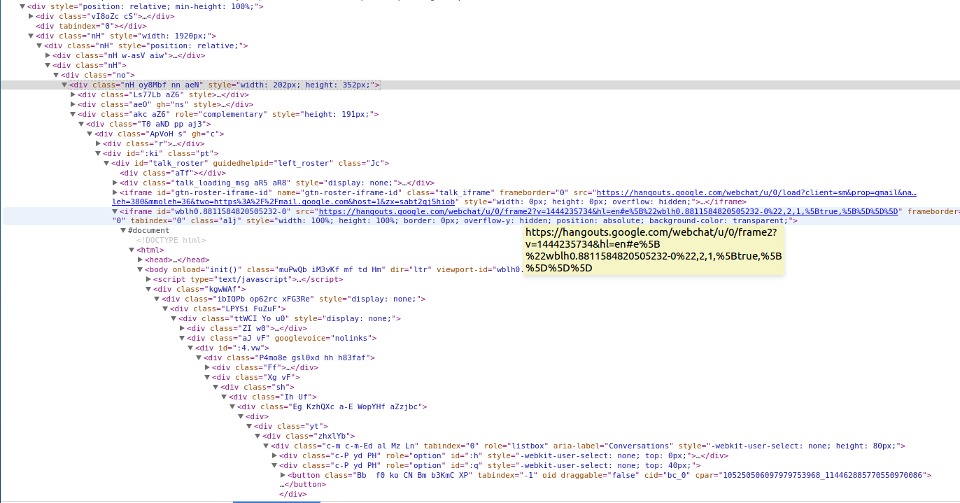
\includegraphics[width=0.75\textwidth]{gmail_example}
		\caption{Gmail DOM structure example}
		\end{figure}
		
		Testing frameworks allow several strategies for locating Web page elements:
		\begin{itemize}
		  \item By id -locates the Web page elements using their id values.
		  \item By name -locates the Web page elements using their name.
		  \item By tag - locates the Web page elements using their tag.
		  \item By class - locates the Web page elements using their class attribute.
		  \item By XPath - combines previous strategies and builds a search
		  path to an element in the DOM.
		\end{itemize}
		
		The choise between these strategies is a tradeoff between effeciency of the
		test and its complexity for developer. The research of Maurizio Leotta
		and Diego Clerissipaper in ``An Industrial Case Study about Web Page Element
		Localization" ``shows that ID-based methods for locating Web page elements are
		better than XPath methods''\cite{selenium4} showing that tests with search by
		Xpath executed more than three times longer than same tests with searching
		elements by Id. According to the same paper ID-based test require less
		maintenance effort, than the XPath-based test suites. In fact using searching by id for static HTML Web pages with small
		amound of elemnetn works well, but having dynamically generated HTML with 
		a lot of elements as in example \ref{fig:gmailexample} brings challengies.
		
		The biggest downside of searching by id strategy, is that every HTML element
		should have a unique ID. If the Web pages has a dynamically generated content,
		for example a table, where amount of rows depends on data, the
		developer has to add some logic to generate ID for each row and also verify
		that new ids do not conflict with already created ones. 
		
		In some circumstances the developer needs to get a set of elements by some
		criteria, for example get all elements with a specific tag or class selector
		and process them in a loop. 
		
		As we can see there is no one solution for searching elements on a Web page,
		which can be used in all cases. The developer should make a solution which
		searching algorithm to use based on requirements, but the testing framework
		should provide the developer different tools to choose from. In the next
		section we present Selenium - a software testing framework for Web
		applications, which allows to create C\&R \ref{sec:captureReplay} and 
        programmable tests \ref{sec:programTests}.Selenium  supports searching
        elements by id,tag, class, Xpath, etc and provides an opportunity to run tests in
        parallel.
		

 